% !TEX root = ../thesis-example.tex
%
\chapter{Analyse von Sprachassistenzsystemen}
\label{sec:analyse}
Im Folgenden wird eine Einleitung in den Aufbau und die Funktionsweise von Sprachassistenten gegeben. Dafür wird zuerst die allgemeine Struktur betrachtet. Außerdem werden die im Folgenden untersuchten Assistenzsysteme vorgestellt und anschließend genauer erläutert, wie sie die Architektur umsetzen. \\
Ein weiterer Betrachtungspunkt sind die aktuellen datenschutzrechtlichen Rahmenbedingungen. Des Weiteren werden auch Bedrohungen analysiert, die für solche System existieren und welche Maßnahmen ergriffen werden können, um diesen vorzubeugen. \\


\section{Architektur von Sprachassistenzsystemen}
\label{sec:analyse:architektur}
QUELLEN NUTZUNG VERBESSERN??
Die allgemeine Architektur von Sprachassistenten folgt gewissen Grundprinzipien, die von  Edu et al. \cite{edu2019smart} sowie Sridhar et al. \cite{sridhar2017evaluating} beschrieben werden und denen die Erläuterungen in diesem Kapitel folgen. Dabei wird die der Fokus der Analyse auf die Software gelegt. Zwar wird auch gewisse Hardware (Mikrofon, Lautsprecher, Analog-Digital-Wandler, Verarbeitungseinheit) benötigt, die Auswahl dieser Bestandteile kann jedoch durch den Anwender getroffen werden und hat nur bedingt Einfluss auf die Unterscheidung der spezifischen Systeme, da die selbe Hardware mit unterschiedlicher Software genutzt werden kann. Die folgenden Erläuterungen folgen dabei den Darstellungen in Abbildung \ref{fig:analyse:allgemeineArchitektur}. 
\begin{figure}
    \centering
    \includegraphics[width=1.0\textwidth]{grafiken/analyse/architektur.png}
    \caption{Übersicht über die allgemeine Verarbeitungspipeline eines Sprachassistenten nach \cite{edu2019smart} }
    \label{fig:analyse:allgemeineArchitektur}
\end{figure}
Die in Bereich I der Abbildung \ref{fig:analyse:allgemeineArchitektur} Aktionen stellen dabei die Interaktion zwischen Nutzer und Assistenzsystem dar. Diesse benötigt einen \texttt{Client}, der die Hardware für Audioein- und Ausgabe besitzt. Damit der Nutzer mit dem System interagieren kann, muss zunächst ein sogenanntes \texttt{Weckwort} (auch \texttt{Signalwort, Wake-Wort, Aktivierungswort}) bezeichnet, gesagt werden. Der der Client mittels eines Mikrofons konstant den Umgebungsgeräuschen lauscht, entdeckt er dieses. Nach dieser Aktivierung beginnt die Aufzeichnung der Audiosignale der durch den Nutzer getätigten Aussage, die als \texttt{Phrase} bezeichnet wird. Daran schließt sich die Analyse dieser Signale an.  \\
Dafür ist eine Umwandlung der Signale in maschinenverständliche Sprache nötig. Damit geht eine Umwandlung der analogen in digitale Signale einher. Um diese weiterverarbeitet werden können, müssen sie in Textform vorliegen. Für diese Transformation kommt ein  \texttt{\ac{STT}}  Umwandler zum Einsatz. Dieser nutzt dafür \ac{NLP}, wodurch zugleich auch Störgeräusche entfernt werden. Auch erlaubt \acs{NLP} es, dass das System akzentbehaftete Sprache verstehen kann \cite{edu2019smart}. Die Filterung der störenden Geräusche wird durchgeführt, bevor es zu einer analog-digital Umwandlung kommt.  Aus dieser digitalisierten Wellenform können durch Analyse von Frequenz und Tonhöhe die einzelnen Bestandteile (Features) herausgefiltert werden. Diese werden danach auf ein zuvor trainiertes Modell angewendet, um so die die entsprechende Textrepräsentation zu ermitteln. Dafür wird immer der aktuelle Signalausschnitt mit dem vorigen und folgenden betrachtet und in einem Lexikon der Wellenformen analysiert, was gesagt wurde. \cite{edu2019smart}\\
Dieser Prozess wird vereinfacht in Abbildung \ref{fig:analyse:speechRecognition} dargestellt. 

\begin{figure}
    \centering
    \includegraphics[width=0.7\textwidth]{grafiken/analyse/speechRecognition.png}
    \caption{Vereinfachte Darstellung der Umwandlung gesprochener Sprache in Text nach \cite{amberkar2018speech}}
    \label{fig:analyse:speechRecognition}
\end{figure}


Im Abschnitt II der Abbildung \ref{fig:analyse:allgemeineArchitektur} erfolgt die Verarbeitung der Anfrage auf Textbasis. Dafür wird diese zuerst an den \texttt{Intent Parser} weitergeleitet. Dieser untersucht den erhaltenen Text auf die gewünschte Aktion, also die Intention des Nutzers, die ausgeführt werden soll. In der einfachsten Umsetzung wird durch diesen Parser eine JSON Ausgabe generiert, die angibt, welcher \texttt{Intent} erkannt wurde. Für diese Erkennung definiert der Entwickler zuvor verschiedene Aussagen, die der Intention zugeordnet werden kann. Mittels dieser Zuordnung wird die gewünschte Aktion hervorgerufen. Außerdem beinhaltet diese Ausgabe die Wahrscheinlichkeit (\texttt{confidence}) dieser Intention und zugehörige Parameter. Für die Beispielanfrage \glqq Wie ist das Wetter in Dresden?\grqq{} ist dies in Abbildung \ref{fig:analyse:jsonBesipiel} dargestellt. Bei einer \texttt{entity} handelt es sich dabei um eine Variable, die für die Durchführung der Handlung zwingend notwendig ist. Würde diese Information im dem Beispiel nicht mit geliefert, könnte dem Nutzer nicht die gewünschte Information geliefert werden. 

\begin{figure}
    \centering
    \begin{verbatim}
    {
        "intent": "wetter",
        "confidence": 0.9577,
        "entity": "Dresden"
    }
    \end{verbatim}
    \caption{Beispiel JSON für Anfrage \glqq Wie ist das Wetter in Dresden?\grqq{}}
    \label{fig:analyse:jsonBesipiel}
\end{figure}

Die im Bereich III der Abbildung \ref{fig:analyse:allgemeineArchitektur} zeigt dabei die Abläufe, wenn die Zuordnung der Anfrage zu einer passenden Anwendung geschehen ist. Diese Anwendungen werden als \texttt{Skills} bezeichnet. Bei diesen handelt es sich um Fähigkeiten, die das System besitzt, um Anfragen zu bewältigen. Ein Skill ist dabei ähnlich einer App auf einem Handy, das heißt, sie stellt eine Schnittstelle zu dem entsprechenden Dienst dar. Außerdem gibt in der Regel einen sogenannten \glqq Marktplatz\grqq{}, auf dem diese Anwendungen angeboten werden. Aus diesen kann sich der Nutzer dann die gewünschten Anwendungen auswählen und seinem System hinzufügen. Es besteht auch die Möglichkeit, sich seine eigenen Skills zu definieren. \\
Außerdem werden die Fähigkeiten in zwei Arten unterschieden. Zum einen sind dies die nativen Skills, welche direkt durch den Hersteller des Assistenzsystems angeboten werden und mit dem System ausgeliefert werden. Außerdem gibt es die Drittanbietekills, die durch eigenständige Entwickler bereitgestellt werden, die unabhängig vom Systemhersteller agieren. \\
Basiert die Analyse auf der zuvor erläuterten Zuweisung von Wahrscheinlichkeiten zu den möglichen Intents, dann wird in nach der abgeschlossenen Analyse derjenige Skill ausgeführt, der die höchste Wahrscheinlichkeit aufweist. In dem in Abbildung \ref{fig:analyse:jsonBesipiel} gezeigten Beispiel wäre dies der Wetter Skill.
Dabei versucht das System zuerst, einen nativen Skill auszuführen. Wenn es keinen solchen gibt, wird versucht, den eines Drittanbieters zu nutzen. Sollte es auch weiterhin keinen passenden Skill geben, wird der Nutzer darüber informiert \cite{edu2019smart}. \\
Nach der Ausführung des Skills kommt es zu einer Antwort an der Aufrufer. Diese liegt dabei zunächst in Textform vor und es kann auch sein, dass diese Antwort nach weiteren Informationen fragt. Im Falle der Kontrolle von Geräten mittels des Sprachassisteten werden entsprechende Befehle durch den Skill an diese weitergeleitet. Bei solchen Geräten kann es sich beispielsweise um verschiedene Teile einer Smart-Home Umgebung handeln. \\
Sofern es eine Antwort an den Nutzer geben soll, muss diese aus der Textform in gesprochene Sprache übersetzt werden. Dargestellt wird dies schematisch im Bereich IV der Abbildung \ref{fig:analyse:allgemeineArchitektur}. Dabei kommt ein \texttt{\ac{TTS}} Umwandler zum Einsatz. Dieser besteht neben einem Sprachmodell auch aus Lautdefinitionen inklusive einer Verslehre, damit es zu einer akustischen Sprachausgabe kommt. Dafür wird der Text in Tokens unterteilt und mittels Textanalyse zu einer Audioausgabe synthetisiert \cite{sridhar2017evaluating}.  In der Regel hat der Nutzer die Möglichkeit, zwischen verschiedenen Stimmen zu wählen. \\



\section{mögliche Assistenzsysteme}
\label{sec:analyse:auswahl}

Da es das Ziel dieser Arbeit ist, ein Konzept für eine unabhängige natürlich-sprachliche Mensch-Roboter-Interaktion zu erstellen, kommen nur solche Sprachassistenzsystem in Frage, die eine Datenverarbeitung erlauben, die auf Infrastruktur eigener Wahl durchgeführt werden kann. Dadurch behält der Nutzer auch die Hoheit über die eigenen Daten, was wiederum unter Datenschutzaspekten ein sehr wichtiger Faktor ist. \\
In diesem Zusammenhang sind zwei verschiedene Projekte von Interesse. Zum Einen \textit{Mycroft AI}, ein komplett quelloffener Sprachassistent. Ein anderes Projekt ist \textit{Snips.ai}, dessen Kernfunktionen frei verfügbar sind und das den Fokus vorrangig auf Datenschutz legt. Gerade der Open-Source Charakter ist wichtig, damit jederzeit Anpassungen an Basisfunktionen vorgenommen werden können, um die Aufgabenerfüllung zu verbessern. Damit die beiden Systeme eingeordnet werden können, wird ein Vergleich mit dem aktuellen Markführer im Bereich Sprachassistenten, Amazon Alexa (siehe Abbildung \ref{fig:analyse:marktanteile}), vorgenommen. 


\begin{figure}[h]
    \centering
    \includegraphics[width=0.6\textwidth]{grafiken/analyse/anteileSprachassistenten.png}
    \caption[Marktanteile der Sprachassistenten 2017]{Marktanteile der Sprachassistenten 2017 \footnotemark}
    \label{fig:analyse:marktanteile}
     
\end{figure}
\footnotetext{https://www.handelsblatt.com/unternehmen/it-medien/elektronikmesse-ifa-siri-alexa-und-google-home-wie-sprachassistenten-die-technikwelt-veraendern/22971046.html [Abgerufen am 11.05.2019]}


\paragraph{Mycroft AI}
Bei Mycroft AI (kurz Mycroft) handelt es sich um einen Open-Source Sprachassistenten, der 2015 erstmals veröffentlicht wurde. Dabei wurde dieser zunächst als komplettes Gerät inklusive Lautsprecher und Mikrofon über Crowdfunding finanziert. Drei Jahre später wurde ein Nachfolgemodell erneut auf dem gleichen Weg finanziert\footnote{https://www.panbachi.de/mycroft-ai-opensource-alternative-zu-alexa-und-co-350/ [Abgerufen am 11.05.2019]}. Zeitgleich mit der Markteinführung des ersten Geräts wurde auch die Software des Systems unter der Apache 2.0 Lizenz frei zur Verfügung gestellt\footnote{https://github.com/MycroftAI/mycroft-core [Abgerufen am 11.05.2019]}. Diese wird direkt in Form eines eigenen Betriebssystems, Picroft, zur Verfügung gestellt. Dabei handelt es sich um einen Ableger von Raspbian. Es ist allerdings auch möglich, die Software mit anderen Linux Derivaten zu betreiben, was allerdings die manuelle Installation weiterer Pakete benötigt. Außerdem wird durch den Hersteller eine Android Anwendung zur Verfügung gestellt. Die Betriebssysteme Windows und MacOS werden mit Stand September 2019 noch nicht unterstützt. \footnote{https://mycroft.ai/get-started/ [Abgerufen am 19.09.2019]} \\
Mycroft zeichnet sich insgesamt besonders durch seine Modularität aus. Somit kann sich der Nutzer für jeden Schritt der Verarbeitung zwischen verschiedener Software entscheiden. Diese umfasst sowohl durch Mycroft entwickelte Software, als auch die von anderen Anbietern. Teilweise werden für den selben Schritt durch Mycroft verschiedene Produkte angeboten, deren Schwerpunkt jeweils unterschiedlich ist \footnote{https://mycroft.ai/documentation/mycroft-software-hardware/ [Abgerufen am 11.05.2019]}. Details zu den verschiedenen Möglichkeiten werden in Kapitel \ref{sec:analyse:spezArch:mycroft} dargestellt.

\paragraph{Snips AI}

Snips AI (kurz Snips) ist eine Sprachassistenzsoftware, die sich dem Schutz der Privatsphäre verschrieben hat. Dabei steht das Architekurprinzip \glqq Privacy-by-Design\grqq{} im Fokus, welches den Datenschutz in den Mittelpunkt der Entwicklung stellt. Außerdem wirbt das Unternehmen damit, dass die Software die \ac{DSGVO} Regularien (siehe Kapitel \ref{sec:analyse:datenschutz:dsgvo}) erfüllt und alle Verarbeitungsschritte direkt auf dem Engerät durchgeführt werden können, wodurch keine Internetverbindung nötig ist \footnote{https://snips.ai/ [Abgerufen am 11.05.2019]}. Das System kann mit allen gängigen Betriebssystemen, außer Windows, benutzt werden. Es werden alle Linux Distributionen sowie MacOS direkt unterstützt, außerdem werden für Android und iOS entsprechende SDKs zur Verfügung gestellt, um eine einfache Integration in die Anwendungen zu ermöglichen \footnote{https://snips.ai/developers/ [Abgerufen am 11.05.2019]}. \\
Allerdings werden durch den Hersteller nicht alle Teile der Software frei zur Verfügung gestellt. Lediglich der Teil zur Verarbeitung der gesprochenen Sprache ist offen gelegt. Zu diesem wurden auch die theoretischen Betrachtungen veröffentlicht veröffentlicht \cite{coucke2018snips}.

\paragraph{Amazon Alexa}

Bei Amazon Alexa (kurz: Alexa) handelt es sich um die Sprachassistenzsoftware von Amazon, welche für die unternehmenseigenen intelligenten Lautsprecher der Echo Reihe  entwickelt wurde. Dieser Service wird über die Cloud zur Verfügung gestellt und erlaubt auch Drittanbietern eigene Funktionen anzubieten\footnote{https://developer.amazon.com/alexa-skills-kit [Abgerufen am 11.05.2019]}. Durch den \ac{AVS} bietet Amazon die Möglichkeit, Alexa direkt in eigene Geräte zu integrieren. Dabei werden mit Android, iOS, macOS, Ubuntu sowie Windows alle gängigen Betriebssysteme offiziell unterstützt. Außerdem kann das System auch direkt mit Raspbian eingesetzt werden. \footnote{https://github.com/alexa/avs-device-sdk/wiki [Abgerufen am 11.05.2019]}


\section{Architekturdetails der einzelnen Systeme}
\label{sec:analyse:spezArch}

In diesem Kapitel wird genauer betrachtet, wir die zuvor vorgestellten System die einzelnen Bestandteile der Sprachverarbeitung umsetzen. Dabei hat sich herausgestellt, dass die Unternehmen nicht immer kommunizieren, wie die einzelnen Verarbeitungsschritte funktionieren. Teilweise werden auch Schritte, die in Kapitel \ref{sec:analyse:architektur} als Einzelschritte betrachtet werden, zu einem zusammengefasst.

\subsection{Mycroft AI}
\label{sec:analyse:spezArch:mycroft}
Mycroft zeichnet sich neben seiner Modularität auch dadurch aus, dass die Software komplett frei zu Verfügung gestellt wird. Dies umfasst eigene Implementierungen für jeden Schritt der Verarbeitung der natürlichen Sprache und auch ein Kooperation mit Mozilla zur Verbesserung des Sprachverständnisses. Außerdem verspricht das Unternehmen durch diese Offenlegung, dass der Nutzer die Hoheit über seine Daten hat und auch keine Daten verkauft oder für Werbezwecke benutzt werden \footnote{https://mycroft.ai/ [Abgerufen am 14.05.2019]}.

\paragraph{Weckworterkennung} Die Weckworterkennung kann mit verschiedenen Engines durchgeführt werden. Zum einen ist dies PocketSphinx \cite{huggins2006pocketsphinx}, welches unterschiedliche Worte auf Basis von Phonemen unterscheidet. Dies ist um die kleinste Einheit von Lauten der gesprochenen Sprache, die eine Unterscheidung zwischen Wörtern zu lässt. Jedoch führt die Tatsache, dass diese in verschiedenen Sprachen unterschiedlich ausgesprochen werden, zu einem Problem. Wenn die interargierende Person nicht in ihrer Muttersprache kommuniziert, kann es zu fehlerhafter Aussprache von Phonemen kommen, wodurch die Worterkennung nur schlecht oder nicht funktioniert. Eine Internetverbindung für die Weckworterkennung wird nicht benötigt.  \cite{amberkar2018speech}\\
Zum anderen kann Snowboy \footnote{https://snowboy.kitt.ai/ [Abgerufen am 14.05.2019]} von KITT.ai eingesetzt werden, welches auf einem neuronalen Netz basiert. Dieses muss entsprechend vor der Nutzung trainiert werden, damit das gewünschte Aktivierungswort erkannt wird. Diese Erkennung kann offline durchgeführt werden, allerdings kann laut Aberkar et al. \cite{amberkar2018speech} nur ein Signalwort trainiert werden. Im Gegensatz zu PocketSphinx ist diese Software nicht Open-Source. \\
Außerdem kann die durch Mycroft entwickelte Engine Precise \footnote{https://mycroft.ai/documentation/precise/ [Abgerufen am 14.05.2019]} eingesetzt werden. Als Basis dient hierfür ein rekurrentes neuronales Netz, das auf Geräuschmuster trainiert wird. Dadurch ist die Erkennung unabhängiger von einer Sprache oder einem Akzent. Genauso wie die beiden anderen Lösungen für diesen Verarbeitungsschritt mit Mycroft, funktioniert Precise ohne Internetverbindung.

\paragraph{Sprache-zu-Text Umwandlung} Für die Sprache-zu-Text Umwandlung sind zwei verschiedene Umsetzungen von größerem Interesse, auch wenn Mycroft prinzipiell die Nutzung vieler auf dem Markt verfügbarer Engines für diese Aufgabe ermöglicht (u.a. Watson STT, Google STT, Wit.ai) \footnote{https://mycroft.ai/documentation/mycroft-software-hardware/ [Abgerufen am 14.05.2019]}. \\
Eines davon ist Kaldi, ein Open-Source Toolkit für Spracherkennung. Dieses zielt darauf ab, in möglichst vielen Umgebungen einsetzbar zu sein und mit Daten des Linguistic Data Consortium zu funktionieren. Dadurch wird eine große Zahl unterschiedlicher Sprachen unterstützt. Außerdem ist den Entwicklern wichtig, dass die Software während der Entwicklung ausgiebig getestet wird. Eine Besonderheit dieser Implementierung ist, dass sie direkt auf dem Endgerät funktioniert und somit keine Internetverbindung benötigt. \cite{povey2011kaldi} \\
Alternativ bietet sich Mozillas \texttt{DeepSpeech} für die Sprache-zu-Text Umwandlung an, dieses Umsetzung wird auch von Mycroft in Form einer Kooperation gefördert \footnote{https://mycroft.ai/blog/deepspeech-update/ [Abgerufen am 14.05.2019]}.  Dieses Projekt basiert auf den theoretischen Überlegungen von Hannun et al.\cite{hannun2014deep}. Durch die Nutzung von Deep Learning ist es dabei möglich, das System kontinuierlich zu verbessern, während der Systemaufbau zeitgleich möglichst einfach bleibt. Beispielsweise müssen durch den Entwickler keine Modelle zur Geräuschfilterung erstellt werden, da das System dies selbst lernt. Außerdem kommt es auch ohne Konzepte wie Phoneme aus, sondern findet selbständig Unterscheidungskriterien. In Tests hat dieses System dabei Fehlerquoten von 6,5\% erreicht, während die menschliche Fehlerrate für die gleichen Daten mit circa 10\% beziffert wird. Die Implementierung durch Mozilla basiert dabei auf dem Machine Learning Framework \texttt{TensorFlow} von Google. Für das Training werden dabei Daten genutzt, die im Rahmen des \glqq Common Voice\grqq{} Projekts gesammelt wurden. \footnote{https://hacks.mozilla.org/2017/11/a-journey-to-10-word-error-rate/ [Abgerufen am 15.05.2019]}\\
DeepSpeech ist ein System, dass für jeden zur freien Verfügung steht und von Mozilla unter Mithilfe der Community ständig weiterentwickelt wird. So stehen im Juni 2019 circa 50 Sprachen zur Verfügung. Dies sind neben bekannten Sprachen wie Englisch oder Deutsch unter anderem auch Katalanisch oder Irisch. \footnote{https://voice.mozilla.org/en [Abgerufen am 03.06.2019]} \\
Besonders an der Verbindung zwischen Mycroft und DeepSpeech ist die Generierung des Mycroft Open Dataset. Mit diesem werden größere Mengen an  zusätzlichen Daten generiert, die als Trainingsdaten zu Verbesserung des Systems eingesetzt werden können. Damit eine Aufzeichnung der Daten geschieht und diese für das Training verwendet werden, muss der Nutzer aktiv der Nutzung für diesen Zweck zustimmen. Standardmäßig werden erfolgt keine Nutzung der Daten. Allerdings kann DeepSpeech aktuell nur mit einer Cloud eingesetzt werden, auch wenn es durch Mycroft Bemühungen gibt, die Komplexität so anzupassen, dass auch ein Einsatz ohne Internetverbindung möglich ist. \footnote{https://mycroft.ai/voice-mycroft-ai/ [Abgerufen am 15.05.2019]}

\paragraph{Intent Parser} Die Erkennung der Intention des Nutzers kann entweder mit Adapt oder Padatious  durchgeführt werden. Ersteres nutzt dabei einen Schlüsselwortabgleich und berechnet daraus einen Wahrscheinlichkeitswert. Anhand dessen wird danach der gewünschte Skill ausgewählt. Dieser Ablauf ist dabei identisch mit dem in Kapitel \ref{sec:analyse:architektur} beschriebenen. \footnote{https://mycroft.ai/documentation/adapt/ [Abgerufen am 20.05.2019]} \\
Ein anderer Ansatz wird mit Padatious verfolgt. Dieser basiert auf einem neuronalen Netz, wofür im Gegenteil zu Adapt keine einzelnen Wörter sondern ganze Sätze genutzt werden. Dadurch ist dieses System flexibler, da der Aufbau der Aussagen keiner starren Struktur folgen muss. \footnote{https://mycroft.ai/documentation/padatious/ [Abgerufen am 20.05.2019]} \\
Bei beiden Ansätzen kann es aber dazu kommen, dass mehr als nur ein Skill den entsprechenden Intent ausführen kann. Aus diesem Grund kommt zusätzlich das Common Play Framework zum Einsatz. Dieses weist den verschiedenen Entitäten unterschiedliche Gewichte zu, wodurch dann die auszuführenden Aktion genauer bestimmt werden kann. \footnote{https://mycroft.ai/documentation/skills/common-play-framework/ [Abgerufen am 20.05.2019]}

\paragraph{Text-zu-Sprache Umwandlung} Für diese Umwandlung von Text in eine akustische Ausgabe, stellt Mycroft zwei verschiedene, selbst entwickelte, Enginges zu Verfügung. Dies sind Mimic TTS und Mimic 2 TTS. Dabei zeichnet sich Mimic durch einen geringen Ressourcenbedarf aus und kann somit direkt auf dem Endgerät eingesetzt werden. Für die Ausgabe stehen zwei verschiedene Stimmen für Englisch zu Verfügung, wobei in der Zukunft noch weitere Sprachen hinzugefügt werden sollen \footnote{https://mycroft.ai/documentation/mimic/ [Abgerufen am 20.05.2019]}. Die Ausgabe entsteht dabei aus der Kombination von verschiedenen kurzen Audioaufnahmen zu den gewünschten Wörtern.\\
Der Nachfolger, Mimic 2 TTS, setzt auf Deep Learning für die Generierung der Sprachausgabe. Dadurch kann das System Eigenschaften der Sprache, wie Betonung oder Rhythmus, besser umsetzen und somit eine menschlichere Ausgabe erzeugen. Allerdings bedarf diese Lösung mehr Rechenleistung, weshalb sie in der Cloud ausgeführt werden muss und somit eine Internetverbind erfordert. \footnote{https://mycroft.ai/blog/mimic-2-is-live/ [Abgerufen am 20.05.2019]}

%\paragraph{Systemanforderungen}
%Es ist möglich, das eigens für den Raspberry Pi entwickelt Betriebssystem auf verschiedenen Modellen dieser Minicomputer Reihe zu installieren. Offiziell ist es bereits möglich, einen Raspberry Pi 2 einzusetzen, auch wenn dieser nur eine langsame Verarbeitung ermöglicht. Da ein Raspberry Pi 3 offiziell einen problemlosen Einsatz erlaubt, können dessen Spezifikation als die Mindestanforderungen betrachtet werden. \footnote{https://mycroft.ai/documentation/picroft/} \\
%Diese sind somit \footnote{https://www.raspberrypi.org/products/raspberry-pi-3-model-b/}:
%\begin{my_list_item}
%    \item CPU: 4x1,2 GHz
%    \item Arbeitsspeicher: 1 GB DDR2
%    \item Speicherplatz: 8 GB
%\end{my_list_item}

\subsection{Snips AI}
\label{sec:analyse:spezArch:snips}

\paragraph{Weckworterkennung} Die Weckworterkennung erfolgt mittels des Service \glqq snips-hotword\grqq{}. Dieser wird direkt durch Snips zur Verfügung gestellt, jedoch gibt das Unternehmen keinen Informationen über die Funktionsweises dieses Dienstes. Für den Nutzer besteht aber die Möglichkeit, eigene Weckwörter zu trainieren.  \footnote{https://docs.snips.ai/articles/platform/wakeword/personal}

\paragraph{Sprache-zu-Text Umwandlung und Intent Parser} Die Umwandlung von gesprochener Sprache in Text sowie die Analyse der dabei entstandenen Ausgabe findet bei Snips mittels eines einzigen Services statt. Die Extraktion des Textes aus der Audioeingabe geschieht dabei, wie in Abbildung \ref{fig:analyse:sprachpipeline} dargestellt, mittels \texttt{\ac{ASR}} statt. Dieser folgt dem prinzipiellen Ablauf, wie er für \ac{STT} in Kapitel \ref{sec:analyse:architektur} beschrieben wird. Dabei wird die Eingabephrase zuerst in eine phonetische Repräsentation umgewandelt, aus der dann wiederum der Text generiert wird. Der Unterschied zu den vorherigen Beschreibungen liegt im Teil der \texttt{\ac{NLU}}. Dabei wird die in Textform vorliegende Aussage den zuvor definierten Intents zugeordnet. Dies geschieht nicht nur mit einer deterministischen, sondern auch mittels einer probabilistischen Unterscheidung der Phrasen und beinhalteter Entitäten. Das bedeutet, es können sowohl solche Sätze verwendet werden, die den Trainingsdaten entsprechen (deterministische Unterscheidung) oder auch diesen ähneln (probabilistische Unterscheidung) um die Nutzerintention zu bestimmen. \cite{coucke2018snips}
\begin{figure}
    \centering
    \includegraphics[width=1.0\textwidth]{grafiken/analyse/spokenlanguagepipeline.png}
    \caption{Verarbeitungspipeline für gesprochene Sprache aus \cite{coucke2018snips} }
    \label{fig:analyse:sprachpipeline}
\end{figure}

\paragraph{Text-zu-Sprache Umwandlung} Standardmäßig erfolgt die Text-zu-Sprache Umwandlung bei Snips offline. Dabei kann zwischen verschiedenen Diensten gewählt werden. Diese können auch ohne Snips auf Linux Distributionen eingesetzt werden. Dabei handelt es sich unter anderem um \glqq picotts\grqq{}, \glqq makerstts\grqq{}, \glqq pico2wave\grqq{}. \footnote{https://medium.com/snips-ai/is-it-google-aiy-nah-its-snips-f67c9dc2139a [Abgerufen am 21.05.2019]} \\
Es können aber auch andere Services für die Audioausgabe eingebunden werden, unter anderem sind dies  Amazon Polly TTS und Google WaveNet TTS. Diese System wiederum benötigen eine Internetverbindung, da die Umwandlung cloudbasiert stattfindet. Außerdem ist es möglich, Mimic von Mycroft einzusetzen. \footnote{https://github.com/snipsco/awesome-snips\#customisations [Abgerufen am 21.05.2019]}

\subsection{Amazon Alexa}
\label{sec:analyse:spezArch:alexa}
Im Mittelpunkt von Amazon Alexa (kurz Alexa) steht der \acf{AVS}. Dieser gibt Zugang zu den cloudbasierten Komponenten von Alexa und ermöglicht eine Integration von Alexa auf unterschiedlichen Endgeräten. Da ein Großteil des Services auf Infrastruktur von Amazon funktioniert, kommen benötigen die Geräte, auf denen dieser Sprachassistent zum Einsatz kommt nur eine geringe Menge an Ressourcen.  \footnote{https://developer.amazon.com/alexa-voice-service [Abgerufen am 23.05.2019]}

\begin{figure}
    \centering
    \includegraphics{grafiken/analyse/alexa_skill.png}
    \caption{Ablauf des Aufrufs eines Skills mit Alexa aus \cite{anke2019integration}}
    \label{fig:analyse:alexaArchitektur}
\end{figure}


\paragraph{Weckworterkennung} Es ist von Amazon vorgesehen, dass sowohl Sensory TrulyHandsfree als auch Snowboy für die Erkennung des Aktivierungswortes eingesetzt werden können \footnote{https://github.com/alexa/avs-device-sdk/wiki/cmake-parameters\#Wake-word-detector}. Snowboy wird Von KITT.ai, einem Unternehmen das inzwischen zu der chinesichen Firma Baidu gehört, zur Verfügung gestellt. Mit diesem Service ist es möglich eigene Weckwörter für Alexa zu nutzen. Die Erkennung selbst wird direkt auf dem Endgerät durchgeführt \footnote{https://snowboy.kitt.ai/ [Abgerufen am 23.05.2019]}.\\
Bei TrulyHandsfree von Sensory handelt es sich um eine Software, die nach Unternehmensangabe die am meisten genutzte Engine für Spracherkennung ist. Diese zeichnet sich besonders durch hohe Genauigkeit, geringen Ressourcenverbrauch sowie Unterstützung vieler Plattformen aus. Dabei ist es möglich, sowohl vordefinierte Weckwörter zu nutzen als auch eigene zu definieren \footnote{https://www.xda-developers.com/sensory-trulyhandsfree-low-power-hotword/ [Abgerufen am 23.05.2019]}.

\paragraph{Sprache-zu-Text Umwandlung} Wie in Abbildung \ref{fig:analyse:alexaArchitektur} dargestellt, findet dieser Umwandlungsschritt vollständig auf Infrastruktur von Amazon statt. Dabei werden mittels \acf{ASR} die nach dem Aktivierungswort getätigten Aussagen automatisch in Text umgewandelt. Dafür kommt der Dienst \glqq Amazon Lex\grqq{} zum Einsatz. Die dabei verwendeten Funktionen wurden zu diesem Zweck zuvor mittels Deep Learning trainiert. \footnote{https://developer.amazon.com/alexa-skills-kit/asr [Abgerufen am 23.05.2019]}


\paragraph{Intent Parser} Die Erkennung des Intents des Nutzers findet mittels Alexa Skill Kit statt. Dieser greift dabei auch auf \acf{NLU} zurück, welches ebenfalls Bestandteil von \ac{AVS} ist und auch auf mittels Deep Learning trainierte Funktionen zurückgreift. In dem Skill Kit werden verschiedene Fähigkeiten definiert, die mit Alexa ausgeführt werden können.
 Außerdem sind die Aussagen festgelegt, die zu der Ausführung des gewünschten Skills führen. Genauere technische Funktionalitäten werden durch Amazon nicht aufgeführt. \footnote{https://developer.amazon.com/docs/custom-skills/create-intents-utterances-and-slots.html [Abgerufen am 23.05.2019]}

\paragraph{Text-zu-Sprache Umwandlung} Die Umwandlung des Textes in gesprochene Wörter geschieht mittels Amazon Polly, welcher wie in Abbildung \ref{fig:analyse:alexaArchitektur} ersichtlich, auch Teil von \ac{AVS} ist. Dieser Service nutzt Deep Learning um eine möglichst menschenähnliche Sprachausgabe zu erzeugen. Diese kann in acht verschiedenen Sprachen mit 28 unterschiedlichen Stimmen erfolgen. \footnote{https://aws.amazon.com/de/polly/ [Abgerufen am 23.05.2019]}


\section{Datenschutz}
\label{sec:analyse:datenschutz}

Im Zusammenhang mit Sprachassistenten stellen sich auch immer datenschutzrechtliche Fragen, da theoretisch ein ununterbrochenes Belauschen der Nutzer möglich ist. Damit diese Fragen beantwortet werden können, ist es nötig, zuerst die aktuelle Rechtslage zu betrachten. Anschließend kann sich potentiellen Gefährdungen des rechtlichen Rahmens sowie möglichen Angriffspunkten auf die Privatsphäre zugewendet werden. Diese Angriffe können dabei auch Manipulationen des Sprachassitenten darstellten. Neben diesen allgemeinen Betrachtungen erfolgt eine Analyse, wie die in Kapitel \ref{sec:analyse:auswahl} vorgestellten Systeme versuchen, diesen Attacken vorzubeugen. 


\subsection{rechtliche Bedingungen}
\label{sec:analyse:datenschutz:dsgvo}
Die bedeutendste rechtliche Grundlage für den Datenschutz innerhalb der \ac{EU} ist die seit dem 25. Mai 2018 geltende \acf{DSGVO}. Deren wesentliches Ziel ist Anpassung der Datenschutzgesetze an die Gegebenheiten des Internetzeitalters, wobei auch Wert auf technologieneutrale Formulierung der Bestimmungen gelegt wurde. \cite{dsgvo} \\
Aus der Perspektive von Sprachassitenten sind die die folgenden Artikel die relvantesten:
\begin{my_list_item}
    \item Artikel 3 \glqq Räumlicher Anwendungsbereich\grqq{}
    \item Artikel 5 \glqq Grundsätze für die Verarbeitung personenbezogener Daten\grqq{}
    \item Artikel 17 \glqq Recht auf Löschung \grqq{}
    \item Artikel 25 \glqq Datenschutz durch Technikgestaltung und durch datenschutzfreundliche Voreinstellungen\grqq{}
\end{my_list_item}

In Artikel 3 wird da Prinzip des Marktortes eingeführt. Dieses bedeutet, dass alle Regeln der \ac{DSGVO} für alle Unternehmen gelten, die in der \ac{EU} geschäftlich aktiv sind. Dabei ist es irrelevant, an welchem Ort sich der Unternehmenssitz befindet. \cite{dsgvoMarktort} \\
Artikel 5 legt fest, dass Daten nur sparsam erhoben werden dürfen (\glqq Datensparsamkeit\grqq{)} und auch nur für zuvor festgelegte Zwecke (\glqq Zweckbindung\grqq{}) \cite{dsgvo}. Diese Daten sind nach Artikel 17 nach der Erfüllung der Aufgabe zu löschen, außerdem kann jederzeit eine Löschung durch die betroffene Person verlangt werden \cite{dsgvoLoschung}. \\
Durch Artikel 25 wird festgelegt, dass der Datenschutz bereits bei der Entwicklung (\glqq Privacy-by-Design\grqq{}) berücksichtigt werden muss. Außerdem sollen standardmäßig solche Einstellungen aktiviert sein, die die Privatsphäre schützen (\glqq Privacy-by-Default\grqq{}). \cite{dsgvo} 

\subsection{mögliche rechtliche Konflikte}
\label{sec:analyse:datenschutz:konflikte}

Die folgenden möglichen rechtlichen Konflikte beziehen sich auf die im Abschnitt \ref{sec:analyse:datenschutz:dsgvo} erläuterten Aspekte der \ac{DSGVO}. Da alle drei betrachteten Systeme offiziell in Deutschland angeboten werden, gelten die in Kapitel \ref{sec:analyse:datenschutz:dsgvo} betrachteten Gesetze aufgrund des Artikels 3 der \ac{DSGVO} auch für diese Sprachassistenten. \\
Konflikte entstehen vor allem mit einer Speicherung der Daten nach der Abarbeitung der Anfrage, da der vom Nutzer benötigte Zweck erfüllt ist. Auch stellt sich die Frage, ob die standardmäßige Speicherung der Daten dem Prinzip \glqq Privacy-by-Default\grqq{} entspricht. Jedoch haben Furey und Blue \cite{furey2018alexa} festgestellt, dass es unter anderem die weitgefasste Regelung der \glqq Verbesserung der Nutzererfahrung\grqq{} gibt. Unter anderem ließe sich die Nutzung von Daten für das Training der Sprachassistenten auf diese Art klassifizieren oder auch personalisierte Werbung die auf Basis dieser Daten angezeigt wird. \cite{furey2018alexa} \\
Sicherlich wurde die Datennutzung durch Anbieter von Sprachassistenten bereits einer tiefgehenden rechtlichen Untersuchung unterzogen. Jedoch kann auch eine rechtliche legitime Nutzung der Daten bei den Nutzern ein Gefühl der Unsicherheit hinterlassen QUELLE. \\
Von Storr und Storr wurde außerdem herausgefunden, dass die in der Cloud befindlichen Daten durch die Anbieter für Analysen mittels künstlicher Intelligenz benutzt werden und zum Teil auch an andere Anbieter weiterverkauft werden \cite{storr2017internet}.


\subsection{mögliche Bedrohungen durch Dritte}
\label{sec:analyse:datenschutz:angriffspunkte}

Die Bedrohungen der Privatsphäre durch Dritte sollen im Folgenden anhand eines Szenarios betrachtet werden. So soll der Nutzer, Alice, einen Sprachassistenten nach dem Wetter fragen. Dieser nutzt dafür einen Skill eines Drittanbieters (Bob), der auch andere Anwendungen zur Verfügung stellt. Für diese Anfrage wird eine Verbindung zur Cloud benötigt. Außerdem ist der Sprachassistent mit SmartHome Geräten von Alice verbunden. \\
Für ein solches Szenario werden durch Chung et al. \cite{chung2017alexa} Angriffsmöglichkeiten geschildert, die von Jacksong et al. \cite{jackson2018study} erweitert werden. 
Diese Angriffe sind in Abbildung \ref{fig:analyse:angriff} dargestellt. 

\begin{figure}
    \centering
    \includegraphics[width=1.0\textwidth]{grafiken/analyse/Angriffe.png}
    \caption{mögliche Angriffspunkte beim Datenaustausch mit der Cloud}
    \label{fig:analyse:angriff}
\end{figure}

\renewcommand{\theenumi}{\roman{enumi}}%
\begin{my_list_num}
  \item ungewollte Aufnahme von Geräuschen
  \item Manipulation des Endgerätes
  \item Abhören der Daten, während sie an die Cloud geschickt werden
  \item Manipulation der Skills
  \item Zugriff auf Daten, die in der Cloud abgelegt sind
\end{my_list_num}

In dem Szenario kann es zur \textit{ungewollte Aufnahme von Geräuschen (i)} kommen, wenn Alice mit einem Freund namens Alexander redet und ihr Sprachassistent wie in dem von der Verbraucherzentrale NRW untersuchten Fall eine Alexa ist. Wenn Alice nun in einem Gespräch die Aussage: \glqq Ich denke, dass Alexander das weiß\grqq{} trifft, kann es durchaus sein, dass auch Alexa sich angesprochen fühlt. Dies war das Ergebnis der Untersuchung durch die Verbraucherzentrale. Diese hat die Reaktion von Alexa auf die vier standardmäßig verfügbaren Weckworte (\glqq Alexa\grqq{}, \glqq Amazon\grqq{}, \glqq Echo\grqq{}, \glqq Computer\grqq{}) sowohl in abgewandelter Form als auch innerhalb eines Satzes betrachtet. So hat die Verwendung des Weckwortes in einem Satz in der Hälfte der Fälle den Assistenten aktiviert. Dies hat zur Folge, dass diese ungewollte Aufnahme auch ausgewertet wird, obwohl dies durch den Nutzer nicht gewünscht ist \cite{verbraucherzentrale}. Dies stellt durchaus auch einen möglichen Konflikt mit der \ac{DSGVO} dar, da die Einwilligung zur Datenverarbeitung nach Artikel 3 in diesem Moment diskutabel ist. \\
Während sich Alice nicht in ihrer Wohnung befindet, möchte nur Eve Zugang zu dieser erhalten. Da Alice unter anderem ihre Wohnungstür über den Sprachassistenten steuert, will Eve diesen dafür manipulieren \footnote{https://opensource.com/article/19/2/mycroft-voice-assistant}. Für diese \textit{Manipulation des Endgerätes (ii)} hat sie zwei Möglichkeiten. Sie kann dies zum einen dadurch versuchen, in dem sie durch ein möglicherweise nicht vollständig geschlossenes Fenster einen entsprechenden Befehl zuruft \cite{haack2017security}. Zum anderen kann sie versuchen, einen \glqq Delfinangriff\grqq{} wie von Roy et al. geschildert durchzuführen. Dabei werden hochfrequente Töne verschickt, die für Menschen nicht hörbar sind, aber trotzdem von den Assistenzsystemen verarbeitet wird. Getestet wurde dies mit gängigen Systemen wie Alexa, Cortana, Siri und konnte zumindest im Umkreis von 1,5m erfolgreich durchgeführt werden \cite{roy2018inaudible}. \\
Außerdem kann Eve Rückschlüsse aus den Daten ziehen  \textit{während diese an die Cloud geschickt werden (iii)}. Zum einen kann sie Nachrichten einfach lesen, falls diese im Klartext versendet werden. Auch wenn diese verschlüsselt sind, kann sie anhand der Nachrichten Informationen über das Nutzungsverhalten von Alice ziehen. Beispielsweise kann sie so herausfinden, wann normalerweise Personen im Haushalt anwesend sind \cite{apthorpe2017smart}.  \\
Auch für Bob stellen sich Möglichkeiten für den Angriff, durch die \textit{Manipulation von Skills (iv)}. So kann es sein, dass die Anwendung von Bob nach außen vertrauenswürdig wirkt, aber für die Ausführung des Skills ein weiterer, manipulierter aufgerufen wird, ohne das Alice dies merkt. Auch kann die Anwendung von Bob mehr Daten anfordern, als für die erfolgreiche Durchführung der Anfrage nötig sind. Möglicherweise gibt Alice die Einwilligung dazu, da sie im Installationsprozess unaufmerksam war \cite{edu2019smart}. Da Bob mehrere Skills anbietet, kann er auch die Daten der verschiedenen Skills aggregieren und somit ein umfassendes Bild von Alice erhalten. Ein sehr ähnliches Szenario wird von Memon und Anwar am Beispiel von Smartphone Apps beschrieben \cite{memon2015colluding}. \\
Für den Hacker Charles ergibt sich auch eine Angriffsmöglichkeit, in dem er auf die \textit{in der Cloud abgelegten Daten zugreift (v)}. Dies ist ein lohnenswertes Ziel da er nur Zugriff auf dieses eine Element benötigt, um an viele sensible Daten gelangen zu können. Diesen Angriff kann er auf verschiedene Arten durchführen, da ein Cloud Zugriff auf unterschiedlichen Wegen möglich ist (z.B. per App oder Web-Access) \cite{modi2013survey}. Besonderes Interesse erzeugen diese Daten aufgrund ihrer Vielfältigkeit. So ist es durchaus möglich, dass ein Nutzer weitere Geräte (z.B. Fitnesstracker) mit dem Sprachassistenten verbindet, welcher diese Daten dann zentral ablegt. Außerdem entsteht durch Verknüpfung dieser Daten, sogenanntes \glqq daisy chaining\grqq{}, ein umfassendes Bild des Nutzers. An diesem sind auch die Hersteller selber interessiert, um ihre Produkte und Werbung besser auch den Nutzer anzupassen \cite{furey2018she}. 


\subsection{Möglichkeiten zur Verhinderung der Angriffe}

Bestimmte Maßnahmen, um Angriffen vorzubeugen, sind beispielswesie der Ort des Assistenzsystem (z.B. nicht in der Nähe von Fenstern) oder das Trennen von der Energiequelle bei Verlassen der Wohnung \cite{jackson2018study} sind nicht geräte- sondern nutzerabhängig. Deshalb sollen Maßnahmen dieser Art im folgenden nicht genauer betrachtet werden, sondern vielmehr, welche Möglichkeiten die in Abschnitt \ref{sec:analyse:auswahl} Systeme bieten, um Angriffe wie in Abschnitt \ref{sec:analyse:datenschutz:angriffspunkte} beschrieben zu verhindern. \\
Um die ungewollte Aufnahme von Geräuschen zu verhindern, bietet es sich einerseits an, das Weckwort so zu verändern, dass es nicht mehr das Standardwort ist \cite{verbraucherzentrale}. Außerdem sind Benachrichtigungen beim Start und Ende der Aufnahme empfehlenswert, da der Nutzer so erfährt, wann Geräusche aufgenommen werden \cite{jackson2018study, edu2019smart}.\\
Die Manipulation des Endgerätes durch hochfrequente Töne lässt von Seiten des Nutzers nur dadurch vermeiden, in dem eine Sprachauthentifizierung genutzt wird. Diese kann einen Nutzer anhand seiner Sprache erkennen und weiß somit, ob dieser die Berechtigung zur Verwendung des Systems hat \cite{edu2019smart}. Dies wird durch die System in Form von HIER DIE MITTEL BESCHREIBEN angeboten. \\
Allerdings kann eine solche Authentifizierung mittels Sprachaufnahmen umgangen werden \cite{chen2017you}. Aus diesem Grund schlagen Feng et al. vor, dass eine Authentifizierung mittels eines tragbaren Sicherheitstokens. Dieser vergleicht die Körpervibrationen mit den gesprochenen Phrasen, wodurch eine Genauigkeit von 97 \% erzielt wurde \cite{feng2017continuous}. Eine offizielle Integration mit den verschiedenen Sprachassistenten gibt es bislang nicht, allerdings wurde das Projekt mit Google Now prototypisch implementiert. Somit muss diese Authentifizierung zuerst durch den Nutzer selbst implementiert werden. Im Wesentlichen muss eine Kommunikation mittels Bluetooth zwischen Assistent und Token stattfinden, die Auswertung selbst findet dann in der Cloud statt.\\
Um jegliche Attacken auf Daten zu unterbinden, die sich in der Cloud befinden, bietet sich das Prinzip der Datensparsamkeit an. Wenn keine Daten an die Cloud geschickt werden, ist keinerlei Zugriff auf diese möglich. Somit muss das Assistenzsystem sämtlich Daten offline verarbeiten. Dies ist mit Mycroft und Snips möglich, bei Alexa bedarf es allerdings einer Verbindung zu der Cloud. \\
Sollte sich eine Kommunikation mit der Cloud nicht umgehen lassen, sollte die Kommunikation minidestens verschlüsselt stattfinden. Wie aber bereits zuvor erwähnt, haben Apthorpe et al. es geschafft, auch aus verschlüsselter Kommunikation ausreichend Informationen zu gewinnen \cite{apthorpe2017smart}. \\
Außerdem werden in dem Fall auch Daten in der Cloud abgespeichert. Deshaöb empfehlen Jackson und Orebaugh, diese Daten regelmäßig auf unerlaubten Zugriff zu kontrollieren oder sie so schnelle wie möglich zu löschen \cite{jackson2018study}. Dies geht bei Alexa ohne Probleme mittels entsprechender App oder aber über den Webzugriff auf das eigene Nutzerkonto. Sowohl bei Snips als auch Mycroft ist dieses Vorgehen nicht nötig, da beide Systeme ohne Internetverbindung funktionieren. \\
Einen effektiven Schutz gegen manipulierte Skills können schlagen sowohl Jackson als auch Edu et el. nicht vor \cite{edu2019smart, jackson2018study}. Auch wird von den Anbietern der Assistenzsoftware kein Schutz vor solchen manipulierten Skills angeboten. \\
Eine Übersicht über die Umsetzbarkeit der verschiedenen Abwehrmaßnahmen mit den jeweiligen Assistenzsystemen gibt die Tabelle \ref{tab:analyse:abwehr}.


\begin{table}[]
    \centering
    \begin{tabular}{c|c|c|c}
         & Mycroft & Snips & Alexa \\
         \hline
         Individuelles Weckwort & \checkmark & \checkmark & \checkmark  \\
         \hline
         Benachrichtigung & \begin{tabular}{@{}c@{}} \checkmark \\durch akustisches Signal \end{tabular} & & \begin{tabular}{@{}c@{}} \checkmark \\hardwareabhängig \end{tabular} \\
         \hline
         Sprachauthentifizierung & X & X & \begin{tabular}{@{}c@{}} \checkmark \\ muss durch Nutzer\\ aktiviert werden \cite{furey2018she} \end{tabular}\\
         \hline
         Sicherheitstoken & \begin{tabular}{@{}c@{}} manuell \\ zu implementieren \end{tabular} & \begin{tabular}{@{}c@{}} manuell \\ zu implementieren \end{tabular} & \begin{tabular}{@{}c@{}} manuell \\ zu implementieren \end{tabular} \\
         \hline
         Verzicht auf Cloud &     \begin{tabular}{@{}c@{}} \checkmark \\ 
         möglich, \\wenn STT auf \\ eigenem Server \end{tabular}
          & \checkmark & X \\
         \hline
         \begin{tabular}{@{}c@{}} Verschlüsselte \\ Kommunikation \end{tabular}& \checkmark & \begin{tabular}{@{}c@{}} nur lokale \\ Verarbeitung \end{tabular} & \checkmark \\
         \hline
         \begin{tabular}{@{}c@{}} Datenspeicherung \\ in Cloud \end{tabular} & X & X & \checkmark \\
         \hline
         Skillverifizierung & & & \\
    \end{tabular}
    \caption{Möglichkeiten zur Umsetzung der Abwehrmaßnahmen}
    \label{tab:analyse:abwehr}
\end{table}

\section{Zusammenfassung}
\label{sec:analyse:zusammenfassung}

In diesem Kapitel wurde zuerst die allgemeine Architektur von Sprachassistenten analysiert. Diese bestehen grundsätzlich aus einem Mikrofon, Lautsprecher und Verarbeitungseinheit. Damit eine Interaktion stattfinden kann, muss der Nutzer das Gerät mittels eines Weckwortes aktivieren, woraufhin es dann zu einer Datenverarbeitung kommt. Mit seiner Aussage kann der Nutzer unterschiedliche, zuvor installierte, Fähigkeiten aufrufen und er erhält im Normalfall eine möglichst natürlich sprachliche Antwort. Anschließend wurden ein OpenSource Sprachassistent (Mycroft), der Marktführer (Alexa) sowie ein datenschutzorientiertes, teilweise quelloffenes System (Snips) auf ihre spezielle Architektur untersucht. Außerdem wurden die datenschutzrechtlichen Beschränkungen im Hinblick auf die \ac{DSGVO} betrachtet. Auch wurde veranschaulicht, welche möglichen Schwachstellen eines Sprachassistenten ein Angreifer ausnutzen kann. Abschließend erfolgte der Blick darauf, wie mit den Systemen solche Angriffe verhindert werden können. \\

THEMA SPRACHIDENTIFIZIERUNG BEI ALEXA (LETZTER ABSATZ) https://www.heise.de/newsticker/meldung/Gutachter-des-Bundestags-sehen-bei-Alexa-Risiken-fuer-Besucher-und-Kinder-4465748.html